\chapter{Training Neural Networks}

Until now, we saw various CNN architectures and the different layers that we can have in a model. But these models must also be trained, in order to obtain a working model. Here, we'll see various methods for training models, and the different tools that get used during training.

\section{Activation Functions}

Nowadays, there is a set of activation functions that are considered to be the avant-guarde of deep learning, but they might change in a few years. Although different, new versions and types of activation functions might come out, the reasoning between them remains mostly the same. But let's define first what an activation function is:

\begin{definition}{Activation Function}
    An \textbf{activation function} is a function which \textbf{determines} whether a given neuron should \textbf{activate} or not by computing the weighted sum $w$ and adding the bias $b$.
\end{definition}

Until now there are a lot of known and used activation functions: some of them are the \textbf{Sigmoid} function, the \textbf{ReLU}, etc... For now, we'll concentrate on the \textbf{sigmoid} activation function.

\begin{definition}{Sigmoid Activation Function}
    The \textbf{sigmoid activation function} is equal to
    \[ \sigma(x) \eq \frac{1}{1 + e^{-x}} \]

    The output of the sigmoid function is in the range $[0, \; 1]$.
\end{definition}

\noindent The sigmoid function was very popular back in the days, mainly because it represented very well when a neuron should "fire" or not. However, it has 3 main problems, which led to the abandonment of this function. The first problem is that \textbf{saturated neurons kill} the \textbf{gradient}. For instance, suppose that we have the following neuron:

\begin{center}
    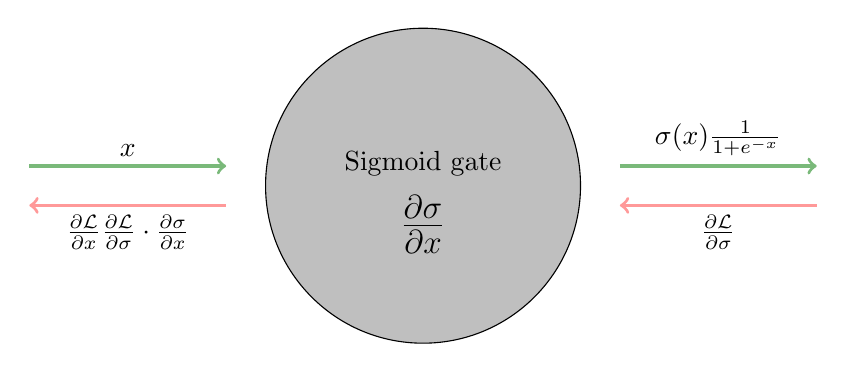
\begin{tikzpicture}
        \filldraw[gray!50, draw=black] (5, 1) circle (2cm) node [anchor = south] {\textcolor{black}{Sigmoid gate}};
        \draw[gray!50] (5, 1) circle (0.1pt) node [anchor = north] {\fontsize{18pt}{18pt}\selectfont\textcolor{black}{$\frac{\partial \sigma}{\partial x}$}};

        \draw[ForestGreen!60, very thick, ->] (0, 1.25) -- (2.5, 1.25);
        \draw[ForestGreen!60] (1.25, 1.25) circle (0.1pt) node [anchor = south] {\textcolor{black}{$x$}};
        \draw[red!40, very thick, <-] (0, 0.75) -- (2.5, 0.75); 
        \draw[red!40] (1.25, 0.75) circle (0.1pt) node [anchor = north] {\textcolor{black}{$\frac{\partial \mathcal{L}}{\partial x} \eq \frac{\partial \mathcal{L}}{\partial \sigma} \cdot \frac{\partial \sigma}{\partial x}$}};

        \draw[ForestGreen!60, very thick, ->] (7.5, 1.25) -- (10, 1.25);
        \draw[ForestGreen!60] (8.75, 1.25) circle (0.1pt) node [anchor = south] {\textcolor{black}{$\sigma(x) \eq \frac{1}{1 + e^{-x}}$}};
        \draw[red!40, very thick, <-] (7.5, 0.75) -- (10, 0.75); 
        \draw[red!40] (8.75, 0.75) circle (0.1pt) node [anchor = north] {\textcolor{black}{$\frac{\partial \mathcal{L}}{\partial \sigma}$}};
    \end{tikzpicture}
\end{center}

More specifically, we define the gradient of the sigmoid functions as follows:
\[ \frac{\partial \sigma}{\partial x} \eq \sigma(x) \cdot (1 - \sigma(x)) \]

Let us try to compute the value of the sigmoid gradient for 3 different values: for $10$, $0$ and $-10$. Let's begin with $x \eq 10$:
\[ \sigma(10) \eq \sim 0 \quad \quad \frac{\partial \sigma}{\partial x} \eq \sigma(10) \cdot (1 - \sigma(10)) \eq 0 \cdot (1 - 0) \eq 0 \]

Now, let's try with $x \eq 0$:
\[ \sigma(0) \eq 0,5 \quad \quad \frac{\partial \sigma}{\partial x} \eq \sigma(0) \cdot (1 - \sigma(0)) \eq 0,5 \cdot (1 - 0,5) \eq 0.25 \]

Finally, let's try with $x \eq -10$:
\[ \sigma(10) \eq \sim 1 \quad \quad \frac{\partial \sigma}{\partial x} \eq \sigma(10) \cdot (1 - \sigma(10)) \eq 1 \cdot (1 - 1) \eq 0 \]

We can see how the result of the gradient is mostly 0, and this clearly results in a problem because when the value of the gradient fill flow down into the network, then the parameters will never update.
\nwl
The second problem with the sigmoid function is that the outputs of the sigmoid are \textbf{not centered in zero}.

\section{Data Preprocessing}

Generally the data can be

\section{Weight Initialization}

\pagebreak

\section{Batch Normalization}

Sometimes, the data, if scattered randomly in the space, can have some patterns that make learning hard for a model. This will make the model not be able to fix a parameter, and would mostly go back and forth between multiple values. If we were able to normalize the data, then we would have a smoother learning. 

\pagebreak

\section{Training and Testing Error}

Whenever we train a model, we usually keep track of two important values: the value of the \textbf{loss function} and the value of the \textbf{accuracy}. We already know how to reduce the value of the loss function, so to use better optimization algorithms. For the accuracy instead, that's a different story: we want to maximize it, but we must avoid \textbf{overfitting}. Generally, we see that there is overfitting when the gap between training accuracy and validation accuracy starts to grow.
\nwl
So how do we deal with this? An idea is to use an \textbf{early stopping} technique: whenever we see that the gap has been augmenting for too much and it also takes greater and greater values, then we want to stop training. This will return a model that could not be overfitting, and it's a technique that should be \textbf{always employed}.
\nwl
If we had the possibility of training multiple models, we can use the \textbf{model ensemble} technique. By training multiple models, we would have for each model different parameters, and at test time we would average the parameters of each model. This would grant, usually a $\sim 2\%$ performance improvement, which may not seem a lot, but it's actually helpful depending on the cases.

\subsection{Regularization and Dropout}

The model ensemble technique works only if we have multiple trainable models, but what can we do to improve the performance of a single model? We can use the \textbf{regularization}. Regularization can be achieved in multiple ways:
\begin{itemize}
    \item with an \textbf{extra term} in the \textbf{loss function};
    \item with the \textbf{dropout};
\end{itemize}

% add loss regularization

The second method, called \textbf{dropout}, is more advanced than the previous method, so adding an extra term to the loss function. For the dropout method, for each forward pass, the output of a neuron is randomly set to 0. This randomness is dictated by a hyperparameter, which is usually $0,5$. This means that around $50\%$ of the neurons will return nothing.
\nwl
But why is this a good idea? Because this makes the network develop a redundant representation, and this way it wouldn't rely on groups of neurons to determine the output. For instance, we define a cat as an animal which has a tail, ears and furr. Say that for each of these features we have a neuron assigned. Now, if we deactivate at random the neuron which detects the ears, if the model learned that a cat must have all of these three features together, then in might not recognize the cat. If we deactivate some neurons instead, then the model will try to recognize the cat also without the feature of the ears.
\nwl
The behaviour of dropout is something that we want to have only during training, not during testing. We want to average out the randomness during test time. So what we can do is the following: if we define with $d(x, \; z)$ the function which determines whether a neuron is deactivated or not, then by taking it's expectation value, we can remove it from the testing of the model.
\[ y \eq \mathbb{E}\left(d(x, \; z)\right) \eq \int p(z) d(x, \; z) \text{d}x \]

This integral is a bit hard to compute though, so how can we compute this without losing time and computational power? We can approximate it. Consider a single neuron $a$:
\begin{itemize}
    \item at test time, the value of $\mathbb{E}[a]$ is equal to
    \[ \mathbb{E}[a] \eq w_1x + w_2y \]
    \item at training time, the value of $\mathbb{E}[a]$ is instead equal to
    \[ \mathbb{E}[a] \eq \frac{1}{4} (w_1x + w_2y) + \frac{1}{4} (w_1x + 0y) + \frac{1}{4} (0x + w_2y) + \frac{1}{4} (0x + 0y) \eq \frac{1}{2} (w_1x + w_2y) \]
\end{itemize}

Notice how the expectation value at training time is just multiplied by the value of the dropout: this makes it much easier for us to compute $\mathbb{E}$.

\subsection{Data Augmentation}

One last regularization method is to perform what is called \textbf{data augmentation}. For this method, 